\section{Numerical results}
\label{sec:results}
Table~\ref{tab:experiments} identifies the historical experiment families. All times are in compactification units, not automatically in units of the black-hole mass. The historical runs in this section were already available for the original manuscript. Section~\ref{sec:telegraph} reports the subsequently authorized telegrapher investigation separately.

\begin{table*}[tp]
\caption{Principal historical evidence families. ``Completed'' means the integrator reached its target, not that the scientific acceptance criteria passed. All listed coupled evolutions use actual scri. Q denotes quadrature shift integration and B denotes the right-biased discrete shift equation. The independent scalar solver is a separate fixed-background control.}
\label{tab:experiments}
\begin{ruledtabular}
\begin{tabular}{p{2.9cm}p{5.2cm}p{3.0cm}p{4.8cm}}
\tcell{Experiment} & \tcell{Gauge / numerical choice} & \tcell{Resolution and duration} & \tcell{Supported interpretation}\\
\hline
\tcell{Finite lapse pulse} & \tcell{$\nu=1$, symmetric restoring; positive variables; B; compensated increments} & \tcell{$2048,4096,8192$; $t=1$} & \tcell{High-order field convergence; finest constraint floor}\\
\tcell{Small lapse pulse} & \tcell{$\nu=1$, symmetric restoring; older primitive-variable Q implementation} & \tcell{$256,512$; $t=10^4$} & \tcell{Long survival; finest continuation paused near $8250$}\\
\tcell{Already-trumpet CMC} & \tcell{Analytic CMC lapse source; symmetric restoring; reference-lapse damping; Q} & \tcell{$256,512,1024$; $t=100$} & \tcell{Small mass drift; separate gauge control}\\
\tcell{Full wormhole prefix} & \tcell{Modified logarithmic source; $\nu=0.25$; AF coefficient chart; Q} & \tcell{$2049,4097,8193$; $t=3.2$} & \tcell{Resolved early physical fields; finest $\HH$ floor}\\
\tcell{Retained wormhole domain} & \tcell{Same gauge; global trumpet metric profile; physical curvature; Q} & \tcell{$1009,2017,4033$; $3.2\leq t\leq10$} & \tcell{All reach target; transient constraint order inadequate}\\
\tcell{Coupled dispersal} & \tcell{$A_\phi=0.058$; $\nu=1$; symmetric restoring; Q} & \tcell{$512,1024,2048$; $t=6$} & \tcell{Convergent mass--flux check; finest component gates pass}\\
\tcell{Collapse trial} & \tcell{$A_\phi=0.07$; $\nu=0.25$; modified source; positive upwind variables; Q} & \tcell{$512,1024,2048$; $t=3$} & \tcell{Large, nonconvergent constraints; failed experiment}
\end{tabular}
\end{ruledtabular}
\end{table*}

\subsection{Minkowski equilibrium and finite lapse pulses}
The reference fields in Eq.~\eqref{eq:reference}, with $\chi=g=1$ and $\Ar=\Th=\Lambda^r=0$, provide an unsubtracted equilibrium check. Analytic cancellation and constant-nullspace differentiation are particularly important here: otherwise derivatives of an order-one background can seed resolution-dependent curvature noise. Successful equilibrium tests do not certify a finite perturbation or the strong-field regime.

The finite-amplitude study starts with the lapse perturbation
\begin{equation}
 \begin{gathered}
 u(0,r)=a_\alpha\exp\left[-\frac{(r^2-r_c^2)^2}{4s^4}\right],
 \\
 (a_\alpha,r_c,s)=(0.1,0.25,0.1),
 \end{gathered}
\end{equation}
and unperturbed geometric data. This is the published-form pulse used as a physical test, not a claim of identical published gauge evolution. On $N=2048,4096,8192$ at fixed CFL, the peak-in-time physical-field difference has observed order $5.0004$ in the bulk and $4.2005$ near scri. Time-RMS orders are $4.9975$ and $4.2089$. Figure~\ref{fig:gauge} shows the underlying differences, including the pulse's passage through the outer region. The approximately fifth-order bulk behavior is consistent with the filter contribution; it should not be described as a uniform sixth-order evolution.

\begin{figure*}[tp]
 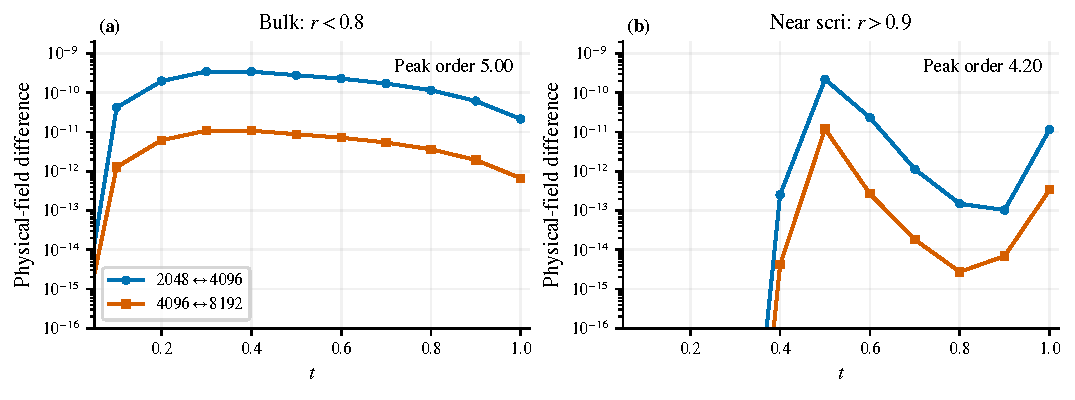
\includegraphics[width=\textwidth]{gauge_convergence}
 \caption{Finite-amplitude lapse pulse with local derivative subtraction and compensated accepted updates. Curves are differences between consecutive resolutions in physical variables at exact common saved times. The peak-difference orders are $5.00$ in the bulk and $4.20$ near scri. Values below the plotted range at early times reflect the initially negligible outer signal, not measured asymptotic convergence. This experiment ends at $t=1$.}
 \label{fig:gauge}
\end{figure*}

The constraint results are more restrictive. Figure~\ref{fig:arithmetic} compares local derivative subtraction with and without compensated accepted increments. At $N=8192$, the peak accepted-state Hamiltonian RMS decreases from $9.99\times10^{-10}$ to $7.88\times10^{-11}$, and the momentum RMS decreases from $7.63\times10^{-10}$ to $5.68\times10^{-11}$. Compensation substantially reduces the arithmetic contamination, but the finest Hamiltonian error still increases relative to $N=4096$. A field-convergence plot alone would miss this limitation.

\begin{figure*}[tp]
 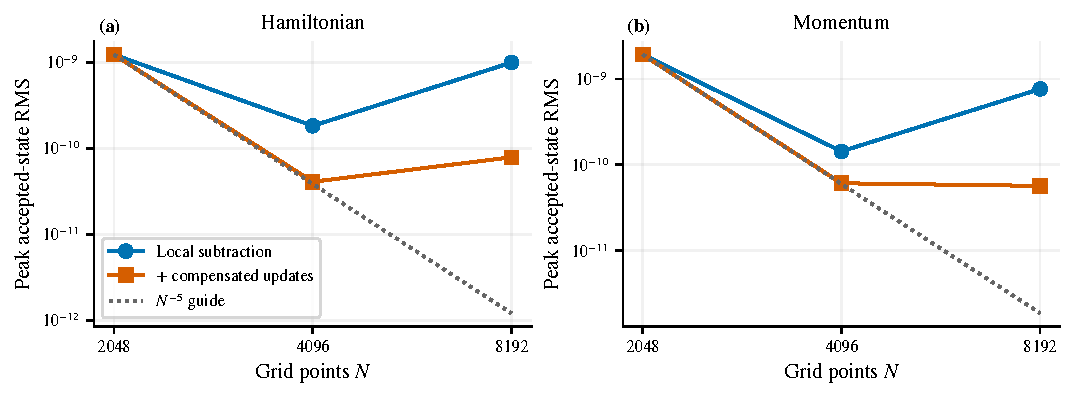
\includegraphics[width=\textwidth]{arithmetic_floor}
 \caption{Peak constraints over all accepted states of the finite pulse on $0\leq t\leq1$. The dotted lines are fifth-order reference slopes, not fits. Compensated updates reduce the finest errors, but do not remove the constraint floor. Intermediate RK trial-state constraints are not substituted for accepted-state accuracy.}
 \label{fig:arithmetic}
\end{figure*}

Independent $N=4096$ controls support separation of time and shift-solve errors from the measured field differences. Halving the timestep changes the final bulk and endpoint fields by $8.07\times10^{-15}$ and $2.44\times10^{-16}$, respectively. These are about $1.17\%$ and $0.070\%$ of the corresponding middle-grid Richardson estimates. Changing the number of banded residual corrections from two to zero or four gives bulk fractions of $1.30\%$ and $1.27\%$, and endpoint fractions below $0.065\%$. One timestep halving does not establish RK4 order; a separate earlier, coarser control resolved RK4. The compensated finest-grid study remains a short-time component result.

The small-amplitude $a_\alpha=10^{-3}$ runs are a different, older implementation family. Two resolutions reached $t=10^4$. The $N=1024$ continuation is paused near $t=8250$, and its accumulated timestamps exhibit the older clock drift. These runs provide long-survival evidence but do not complete a three-resolution long-duration assessment of the later $a_\alpha=0.1$ scheme. Compatible independent constraint perturbations and resolution-scaled noise have also been exercised. Smooth supported constraint perturbations at $N=128,256,512$ reach $t=10$ and decay. The original fixed-amplitude nodal-noise sequence reaches $t=6$, but its finest-grid $\Th$ amplification, $129.5$, exceeds the declared per-component limit of $100$. This remains a failed test. High-frequency metric noise enters $\HH$ through second derivatives, so a fixed nodal amplitude does not bound the mixed-derivative perturbation size uniformly under refinement.

A separately specified, derivative-balanced dataset scales the $\chi$ perturbation as $h^2$ and the independent curvature, $\Kh$, $\Th$, and connection perturbations as $h$. With amplitude parameter $10^{-5}$ and seed $7419$, all four grids $N=128,256,512,1024$ reach $t=6$ and pass the boundary, positivity, component-amplification, and final-decay gates. On the finest grid the peak amplification factors for $(\HH,\MM,\Th,Z_r)$ are approximately $(1.46,1.00,1.15,7.20)$, and the final-to-initial ratios are below $3.1\times10^{-7}$. This is a distinct perturbation experiment, not a retrospective pass for unscaled noise or a spatial-convergence study of fixed continuum data. A comprehensive long-duration robust-stability assessment is still absent.

\subsection{Endpoint and discrete-shift failures}
\label{sec:endpoint-failures}
The naive l'Hopital endpoint treatment has a readily identifiable discrete failure. The scalar model $T_t=-cT/\Omega$, extended at scri by $T_t=cD_rT$, contains a positive diagonal endpoint contribution. In the recorded $N=24$ comparison, the full endpoint-localized mode grows at approximately $232.44$, close to the model value $232.60$. This does not contradict a continuum statement restricted to compatible weighted data. It demonstrates that the unrestricted nodal phase is larger than that continuum phase. Extrapolating the combined quotient reduced, but did not remove, the observed instability.

A second failure arises even when the discrete elliptic system is solved accurately. The centered shift-ODE variant fails the finite pulse near $t=0.7073$, $0.2970$, and $0.1055$ at $N=512,1024,2048$. Timestep halving does not repair the middle-grid failure. Its coupled finite-grid Jacobian has growing outer-localized modes; the dominant real part reaches $44.66$ at $N=512$. The right-biased variant has a dominant real part near $-0.706$ on the tested grids [Fig.~\ref{fig:endpoint}(a)]. These spectra diagnose the tested discrete systems; they are not continuum or nonlinear stability proofs.

Finally, a successful final-time convergence check can be misleading. The original right-biased $512/1024/2048$ study gives endpoint order $4.82$ at $t=1$, but only about $1.28$ at $t=0.5$ [Fig.~\ref{fig:endpoint}(b)]. The fixed-grid timestep difference at that transient is $5.76\times10^{-14}$, far below the spatial discrepancy. Refinement and arithmetic controls, rather than a new time integrator, were therefore the relevant next tests. The finer result in Fig.~\ref{fig:gauge} improves this behavior, without retroactively making the coarse experiment acceptable.

\begin{figure*}[tp]
 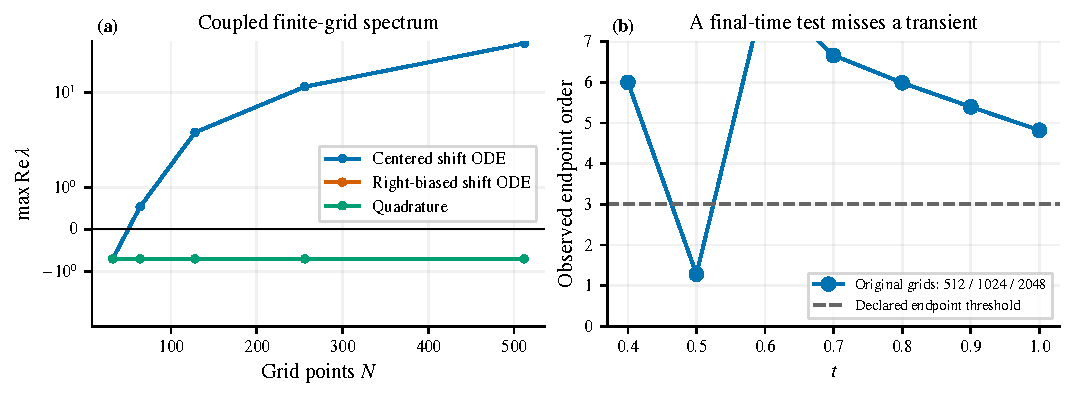
\includegraphics[width=\textwidth]{endpoint_failures}
 \caption{Two distinct endpoint-related failures. (a) Dominant real eigenvalue of the coupled finite-grid Jacobian; the vertical scale is symmetric logarithmic. An accurately solved centered shift matrix can still destabilize evolution. (b) Endpoint self-convergence order of the original finite-pulse grids at exact common snapshots. The transient falls below the predeclared order-three threshold despite good final-time convergence. The panels use different diagnostics and do not establish a nonlinear energy estimate.}
 \label{fig:endpoint}
\end{figure*}

\subsection{Already-trumpet control}
\label{sec:cmc}
Stationary Schwarzschild CMC data provide a geometric control independent of the wormhole construction. Let
\begin{equation}
 \mathcal J=R-\frac C{R^2},\qquad
 f_R=1-\frac{2M}{R}+(\mathcal J)^2.
\end{equation}
Here $\mathcal J$ is the physical normal derivative of areal radius. A double zero of $f_R$ defines the trumpet end $R_0$, with
\begin{equation}
 C=R_0^2\sqrt{R_0^2+1/3},\qquad
 M=R_0^3+\frac{2R_0}{3}-C.
\end{equation}
The fields are $\chi=[r/(\Omega R)]^2$, $\Ar=-2C/(\Omega R^3)$, $\Kh=-3$, $\alpha=\Omega\sqrt{f_R}$, and $\beta=-r\mathcal J/R$. The isotropic map is evaluated after analytic removal of its logarithmic double-root singularity. Initial native constraints are below $6.5\times10^{-12}$ and the geometric rates below $4.5\times10^{-13}$ in the recorded audit.

The evolved control uses a finite cutoff $r_{\min}=0.03$, an analytic \emph{lapse-only} source adapted to this CMC geometry, symmetric restoring, and reference-lapse damping. No numerical Schwarzschild RHS is subtracted. All three grids reach $t=100$. At $N=1024$, the peak Hamiltonian and momentum RMS values are $1.11\times10^{-9}$ and $1.69\times10^{-9}$, with relative horizon-mass drift $1.37\times10^{-12}$. Figure~\ref{fig:cmc} also shows that the finest constraints are not uniformly smaller than the middle-grid values. Earlier multiplicative-source excision controls halted when the gauge characteristic became incoming; constant damping also allowed greater late-time growth. The successful duration of this specialized control does not validate the main Minkowski-reference wormhole experiment.

\begin{figure*}[tp]
 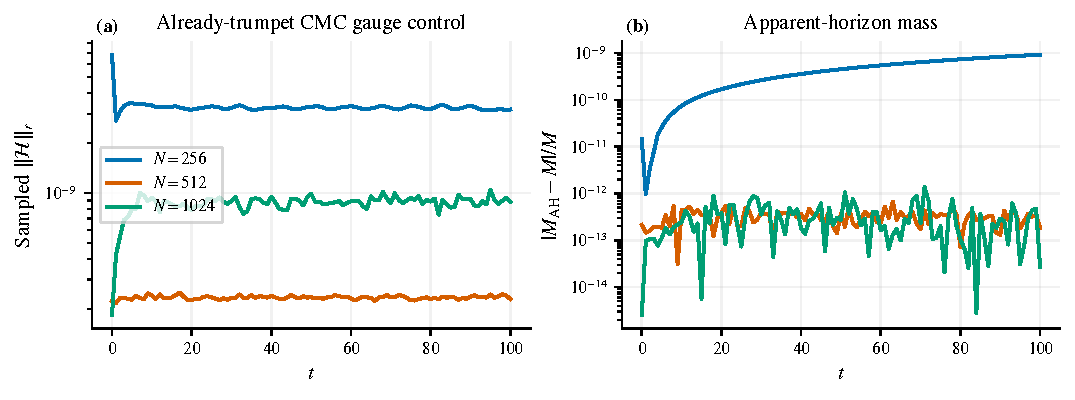
\includegraphics[width=\textwidth]{cmc_control}
 \caption{Already-trumpet CMC control, $M=1/3$, with an analytic CMC lapse source and reference-lapse damping. Sampled Hamiltonian RMS and relative apparent-horizon mass error remain small through $t=100$, but the finest Hamiltonian curve shows a floor/upturn. Isolated zero mass errors are omitted on the logarithmic axis. These data are neither wormhole-to-trumpet evolution nor the main Minkowski-reference gauge.}
 \label{fig:cmc}
\end{figure*}

\subsection{Genuine wormhole data and strong-field fronts}
\label{sec:wormhole}
The wormhole data are constructed as a slice of Schwarzschild spacetime rather than by compactifying time-symmetric data and assuming hyperboloidal asymptotics. With $F_S=1-2M/R$, prescribe the physical normal radius derivative $H(R)=s(R)R$, where the smooth outer-branch switch rises from zero at $4M$ to one at $8M$. Then
\begin{equation}
 \begin{gathered}
 h_R=\frac{H}{F_S\sqrt{F_S+H^2}},\quad
 \widetilde\gamma_{RR}=\frac1{F_S+H^2},\\
 K_R{}^R=-H_R,\quad K_\theta{}^\theta=-H/R.
 \end{gathered}
\end{equation}
The inner region remains the two-ended isotropic wormhole,
\begin{equation}
 R=\rho\left(1+\frac{M}{2\rho}\right)^2,\qquad
 \widetilde\alpha=\left(1+\frac{M}{2\rho}\right)^{-2}.
\end{equation}
An isotropic compactifying map gives $g=1$ and joins this interior to a hyperboloidal exterior. The second asymptotically flat end is excluded from the outer height transition. The construction is analytically vacuum; the recorded initial-data audit gives Hamiltonian and momentum errors below $2.3\times10^{-13}$ and $3.9\times10^{-14}$ at its tested points.

For $M=1/3$ and $\nu=1$, the modified logarithmic source still produces a sharp inward-moving front. At $t=2.5$, the physical-lapse gradient near $r=0.119$ increases from $22.86$ to $40.65$ to $76.92$ as $N$ increases from $513$ to $1025$ to $2049$. The trace develops a narrow negative spike, and local Hamiltonian maxima increase from $0.409$ to $0.654$ to $0.974$ (Fig.~\ref{fig:front}). The front subsequently moves inward. These data rule out a smooth, resolved convergence interpretation of that trial. They support a gauge-steepening diagnosis, but do not prove a gauge-shock theorem for this spherical, nonlocal-shift system. Results for simpler slicing systems\cite{Alcubierre2005,BaumgarteHilditch2022} motivate this interpretation without establishing it here.

\begin{figure*}[tp]
 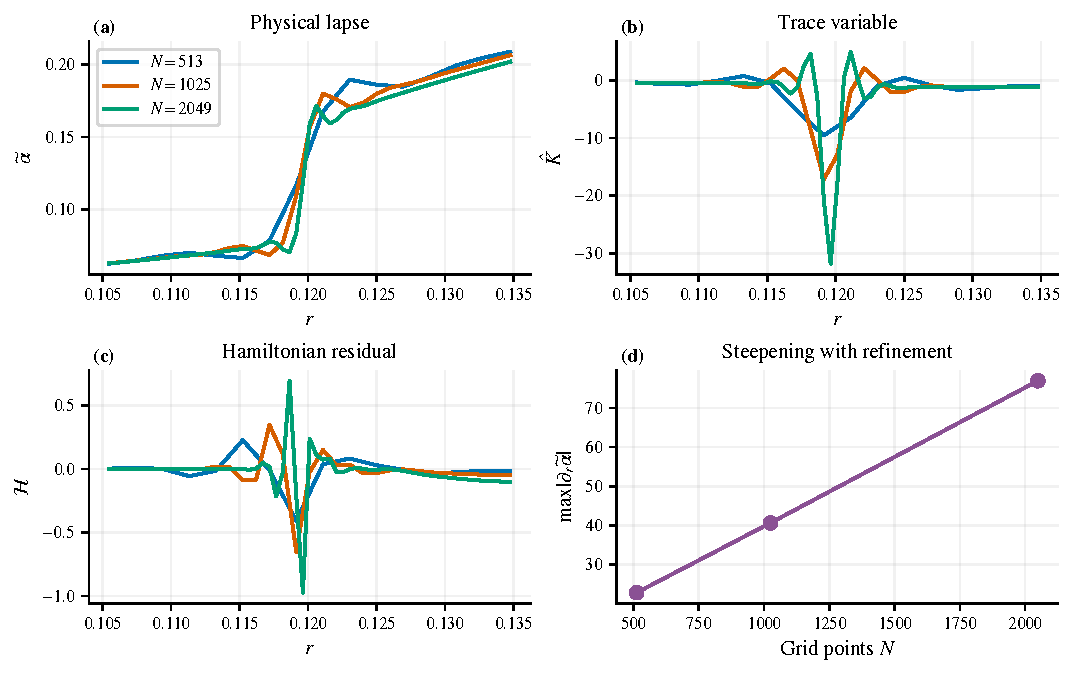
\includegraphics[width=\textwidth]{wormhole_front}
 \caption{Failed $\nu=1$ wormhole trial with the modified logarithmic source, shown at the exact saved time $t=2.5$. The physical lapse steepens, $\Kh$ develops a narrow spike, and the local Hamiltonian error grows under refinement. The gradient diagnostic in (d) uses second-order differentiation of saved profiles; it is not the evolution stencil. This is evidence of unresolved steepening, not a proof of a continuum shock.}
 \label{fig:front}
\end{figure*}

Reducing the positive logarithmic coefficient to $\nu=0.25$ improves the early evolution. Full-domain prefixes on $N=2049,4097,8193$ through $t=3.2$ give peak physical-field self-convergence orders $5.50$ in the bulk and $5.86$ near scri. The peak accepted momentum RMS decreases as $2.77\times10^{-5}$, $1.47\times10^{-6}$, and $6.87\times10^{-8}$. The Hamiltonian RMS, however, is $1.01\times10^{-7}$, $3.00\times10^{-9}$, and $5.37\times10^{-9}$; the finest upturn remains visible. These are prefix results only. An existing exact-source continuation of $N=4097$ reaches $t=3.6$, but does not supply the missing full long-duration study.

\subsection{Causal retained domains: improvement without acceptance}
The retained-domain comparison transfers the saved $t=3.2$ wormhole states to $r\geq1/64$, using the global profile in Eq.~\eqref{eq:trumpet-chart}. It retains $1009$, $2017$, and $4033$ points from full grids of $1025$, $2049$, and $4097$, respectively. The main gauge remains Minkowski-referenced, with $\nu=0.25$, the modified logarithmic source, and constant damping. All runs reach $t=10$ and remain outward-characteristic at the cutoff. Their transient constraint accuracy is insufficient (Table~\ref{tab:domain}).

\begin{table}[tbp]
\caption{Retained-domain peak accepted-state constraints on $3.2\leq t\leq10$. These maxima include the early transient.}
\label{tab:domain}
\begin{ruledtabular}
\begin{tabular}{rcc}
$N$ & $\max_t\normr{\HH}$ & $\max_t\normr{\MM}$\\
\hline
1009 & $5.45\times10^{-4}$ & $1.46\times10^{-3}$\\
2017 & $2.10\times10^{-4}$ & $5.25\times10^{-4}$\\
4033 & $4.63\times10^{-5}$ & $1.20\times10^{-4}$
\end{tabular}
\end{ruledtabular}
\end{table}

RMS Hamiltonian pair orders are approximately $1.38$ and $2.18$, with momentum orders $1.47$ and $2.12$. Bulk maximum-norm orders are lower still. Clean late-time constraints or an accurate exterior mass therefore do not establish a successful experiment. Figure~\ref{fig:domain} retains the transient and shows a distinct representation effect: the compact metric profile introduces late constraint structure near $r\simeq0.112$, inside its transition region. The same-grid global profile largely removes this artifact. The transient remains in both, so eliminating the profile artifact is not a complete repair.

The earlier finite-cutoff and asymptotic-chart failures also limit interpretation. An outward physical light cone alone was insufficient because the gauge cone could be incoming. A gauge-only Robin treatment later halted when a physical characteristic entered. Stronger dissipation, SBP6/3 differentiation, and a tapered cutoff filter did not produce an accepted full wormhole evolution. For finite time the full continuum wormhole retains an asymptotically flat inner core; a trumpet limit must be established outside that shrinking core using lapse collapse, limiting areal radius, proper-distance behavior, and invariant convergence. That demonstration remains unfinished.

\begin{figure*}[tp]
 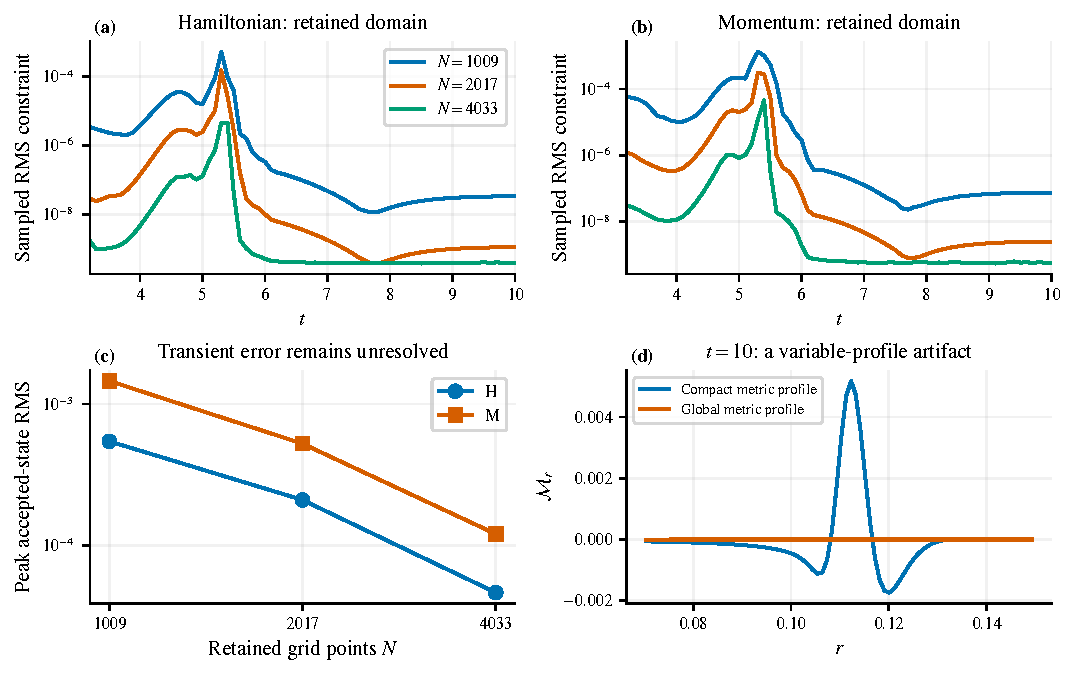
\includegraphics[width=\textwidth]{retained_domain}
 \caption{Completed retained-domain experiments with the global metric profile and $\nu=0.25$. Panels (a,b) show saved-time RMS constraints, whereas (c) uses maxima over every accepted state; narrow peaks can exceed the saved-time curves. The measured orders remain inadequate. Panel (d) isolates the late compact-profile artifact using two $N=1009$ runs with identical physical initial fields and gauge sources. These plots exclude the excised region and cannot replace assessment of the full preceding wormhole trajectory.}
 \label{fig:domain}
\end{figure*}

\subsection{Scalar propagation, dispersal, and failed collapse}
An independent fixed-Minkowski scalar solver provides a preliminary propagation oracle. The physical analytic solution is an ingoing/outgoing spherical wave of the form $\phi=[F(T-R)-F(T+R)]/R$. This separate second-order characteristic discretization gives weighted-field orders $1.96$ and $2.00$ and scri orders $1.90$ and $1.98$ on $N=200,400,800$ through $t=3$ [Fig.~\ref{fig:scalar}(a)]. It neither tests the full coupled geometry nor establishes high-order accuracy of the evolution code.

The coupled subcritical data use
\begin{equation}
 \phi(0,r)=A_\phi\exp\left[-\frac{(r^2-0.25^2)^2}{4(0.1)^4}\right],
 \qquad A_\phi=0.058,
\end{equation}
with the constraint solve described above. The initial mass is approximately $0.105734092466$. At $t=6$, $|M_0-E_{\rm rad}|$ is $6.99\times10^{-6}$, $2.53\times10^{-7}$, and $8.19\times10^{-9}$ on $N=512,1024,2048$. The residual mass sampled at $r=0.9$ is about $1.9\times10^{-11}$, much smaller than the finest budget discrepancy. The two budget-error ratios correspond to orders about $4.79$ and $4.94$.

The finest run has peak scri pole residue $1.26\times10^{-8}$ and a conservative nonaffinity bound $6\max|\kappa_B|=5.80\times10^{-8}$, below the specified $10^{-7}$ bound. The two coarser runs fail some boundary/affinity gates. We use the RK-integrated flux for this comparison: quadrature of sparsely saved flux samples can underresolve the pulse by much more than the reported budget error. The result is a short-time coupled dispersal check, not a measured tail or a completed principal study with all independent controls.

The collapse attempts are unsuccessful. The latest positive-variable, upwind, $A_\phi=0.07$ trial reaches $t=3$ at all three resolutions, but its all-stage Hamiltonian RMS peaks are $3.71\times10^8$, $3.05\times10^{10}$, and $1.94\times10^{10}$. Sampled histories are shown in Fig.~\ref{fig:scalar}(d). Numerical survival and any apparent-horizon crossing in such a trajectory cannot be interpreted as reliable black-hole formation. Earlier source and transport variants also failed. No coupled black-hole scalar perturbation, quasinormal frequency, or late-time decay exponent is extracted from these data. Those physical tests, including neutral limits of later scalar studies\cite{Alvares2026}, remain future work.

\begin{figure*}[tp]
 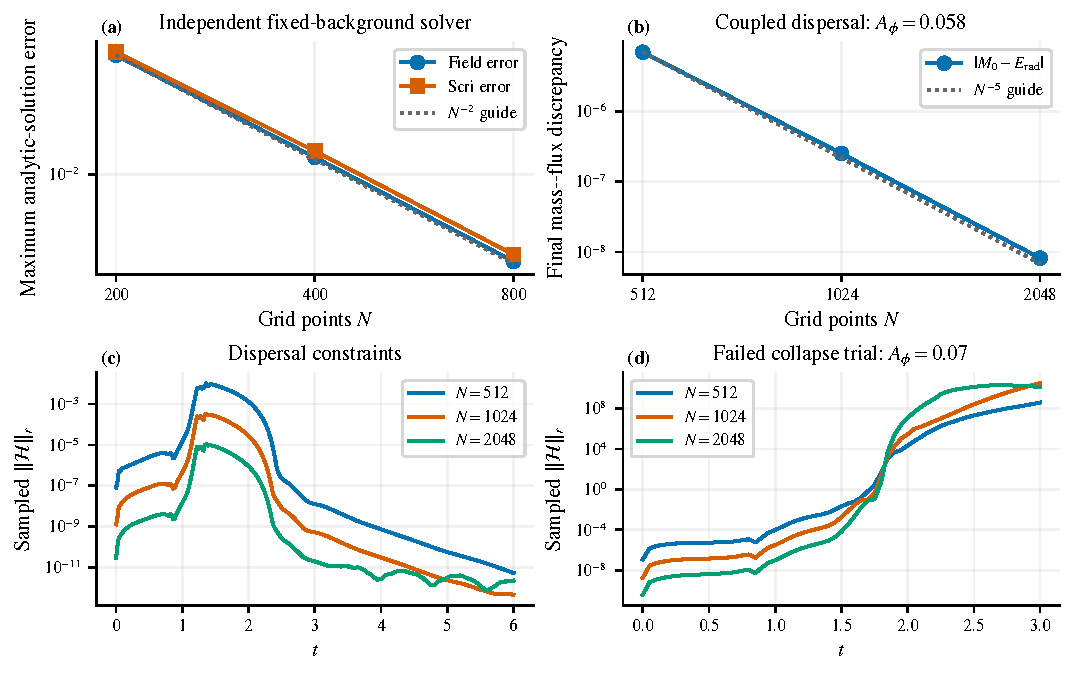
\includegraphics[width=\textwidth]{scalar_results}
 \caption{Scalar evidence with its scope kept explicit. (a) Independent second-order fixed-background oracle. (b) Coupled subcritical mass--flux discrepancy at $t=6$; the dotted slope is a guide. (c) Sampled coupled dispersal constraints. (d) A different, failed $A_\phi=0.07$ collapse family with enormous constraints. Panels (c,d) use different lapse-source/variable choices, so their contrast is not a controlled amplitude-only comparison. Reaching the target time in (d) is not evidence of accurate collapse.}
 \label{fig:scalar}
\end{figure*}
